\documentclass[11pt,a4paper]{article}
\usepackage[margin=2cm]{geometry}
\usepackage{graphicx}
\usepackage{xcolor}
\usepackage{tikz}
\usepackage{amsmath}
\usepackage{amssymb}
\usepackage{enumitem}
\usepackage{tcolorbox}
\usepackage{multicol}
\usepackage{fancyhdr}
\usepackage{hyperref}
\usepackage{array}
\usepackage{tabularx}
\usepackage{booktabs}

% Define colors from slides
\definecolor{mlblue}{HTML}{1f77b4}
\definecolor{mlorange}{HTML}{ff7f0e}
\definecolor{mlgreen}{HTML}{2ca02c}
\definecolor{mlred}{HTML}{d62728}
\definecolor{mlpurple}{HTML}{9467bd}
\definecolor{mlgray}{HTML}{7f7f7f}
\definecolor{mlyellow}{HTML}{bcbd22}
\definecolor{mlcyan}{HTML}{17becf}

% TikZ libraries
\usetikzlibrary{shapes.geometric, arrows, positioning, calc, shadows, patterns}

% Page style
\pagestyle{fancy}
\fancyhf{}
\lhead{\textcolor{mlblue}{\textbf{ML for Innovation}}}
\rhead{\textcolor{mlgray}{Discovery Journey}}
\cfoot{\thepage}
\renewcommand{\headrulewidth}{0.4pt}
\setlength{\headheight}{14pt}

% Custom environments
\newtcolorbox{discoverybox}[2]{
    colback=#1!10, 
    colframe=#1!50, 
    title={#2},
    fonttitle=\bfseries,
    boxsep=5pt,
    arc=2pt
}

\newtcolorbox{exercisebox}[2]{
    colback=white, 
    colframe=#1!50, 
    title={Exercise: #2},
    fonttitle=\bfseries,
    boxsep=5pt,
    arc=2pt
}

\newtcolorbox{didyouknow}{
    colback=mlyellow!10,
    colframe=mlyellow!70,
    title={\textbf{Did You Know?}},
    fonttitle=\bfseries,
    boxsep=5pt,
    arc=2pt
}

\newtcolorbox{challenge}{
    colback=mlred!10,
    colframe=mlred!70,
    title={\textbf{Challenge}},
    fonttitle=\bfseries,
    boxsep=5pt,
    arc=2pt
}

\newtcolorbox{casestudy}{
    colback=mlcyan!10,
    colframe=mlcyan!70,
    title={\textbf{Real Case Study}},
    fonttitle=\bfseries,
    boxsep=5pt,
    arc=2pt
}

\begin{document}

% PAGE 1: Enhanced Cover Page
\thispagestyle{empty}
\begin{center}
\vspace*{1cm}

{\Huge \textcolor{mlblue}{\textbf{Machine Learning for Innovation}}}

\vspace{0.5cm}

{\LARGE \textcolor{mlpurple}{A Discovery Journey with Real Data}}

\vspace{1.5cm}

\begin{challenge}
\Large \textbf{Can You Beat the Algorithm?}\\[0.5cm]
\normalsize Inside: 8 challenges where human intuition fails\\
and machine learning reveals hidden innovation patterns
\end{challenge}

\vspace{1cm}

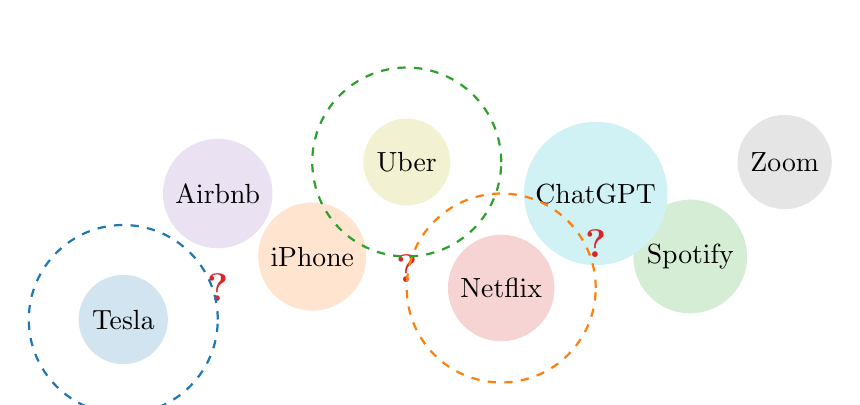
\begin{tikzpicture}[scale=0.8]
% Draw innovation icons in a scattered pattern
\node[circle, fill=mlblue!20, minimum size=1cm] at (0,0) {Tesla};
\node[circle, fill=mlorange!20, minimum size=1cm] at (3,1) {iPhone};
\node[circle, fill=mlred!20, minimum size=1cm] at (6,0.5) {Netflix};
\node[circle, fill=mlgreen!20, minimum size=1cm] at (9,1) {Spotify};
\node[circle, fill=mlpurple!20, minimum size=1cm] at (1.5,2) {Airbnb};
\node[circle, fill=mlyellow!20, minimum size=1cm] at (4.5,2.5) {Uber};
\node[circle, fill=mlcyan!20, minimum size=1cm] at (7.5,2) {ChatGPT};
\node[circle, fill=mlgray!20, minimum size=1cm] at (10.5,2.5) {Zoom};

% Draw question marks between them
\node[text=mlred, font=\Large\bfseries] at (1.5,0.5) {?};
\node[text=mlred, font=\Large\bfseries] at (4.5,0.8) {?};
\node[text=mlred, font=\Large\bfseries] at (7.5,1.2) {?};

% Draw clustering circles appearing
\draw[mlblue, thick, dashed] (0,0) circle (1.5cm);
\draw[mlorange, thick, dashed] (6,0.5) circle (1.5cm);
\draw[mlgreen, thick, dashed] (4.5,2.5) circle (1.5cm);
\end{tikzpicture}

\vspace{2cm}

\begin{tcolorbox}[colback=white, colframe=mlblue!50, width=0.7\textwidth]
\Large
\textbf{Name:} \hrulefill

\vspace{0.5cm}

\textbf{Date:} \hrulefill

\vspace{0.5cm}

\textbf{Your Field:} \hrulefill
\end{tcolorbox}

\vspace{1cm}

\begin{didyouknow}
Companies using ML for innovation pattern discovery are \textbf{2.3x more likely} to be industry leaders
\end{didyouknow}

\end{center}

\newpage

% PAGE 2: Real Innovation Grouping Challenge
\section*{Challenge 1: Group These Real Innovations}

\begin{exercisebox}{mlred}{Beat the Algorithm - Round 1}
Below are 20 real innovations. Group them into 4 categories. You have 3 minutes!
\end{exercisebox}

\begin{center}
\begin{tabular}{cccc}
\fbox{\parbox{3.5cm}{\centering\small\textbf{Tesla Model 3}\\Electric Vehicle\\2017}} & 
\fbox{\parbox{3.5cm}{\centering\small\textbf{iPhone}\\Smartphone\\2007}} & 
\fbox{\parbox{3.5cm}{\centering\small\textbf{Netflix}\\Streaming\\1997}} & 
\fbox{\parbox{3.5cm}{\centering\small\textbf{Airbnb}\\Sharing Economy\\2008}} \\[0.5cm]

\fbox{\parbox{3.5cm}{\centering\small\textbf{Spotify}\\Music Streaming\\2006}} & 
\fbox{\parbox{3.5cm}{\centering\small\textbf{Uber}\\Ride Sharing\\2009}} & 
\fbox{\parbox{3.5cm}{\centering\small\textbf{ChatGPT}\\AI Assistant\\2022}} & 
\fbox{\parbox{3.5cm}{\centering\small\textbf{Zoom}\\Video Conferencing\\2011}} \\[0.5cm]

\fbox{\parbox{3.5cm}{\centering\small\textbf{Instagram}\\Social Media\\2010}} & 
\fbox{\parbox{3.5cm}{\centering\small\textbf{PayPal}\\Digital Payment\\1998}} & 
\fbox{\parbox{3.5cm}{\centering\small\textbf{Amazon Prime}\\Subscription\\2005}} & 
\fbox{\parbox{3.5cm}{\centering\small\textbf{Google Maps}\\Navigation\\2005}} \\[0.5cm]

\fbox{\parbox{3.5cm}{\centering\small\textbf{WhatsApp}\\Messaging\\2009}} & 
\fbox{\parbox{3.5cm}{\centering\small\textbf{Bitcoin}\\Cryptocurrency\\2009}} & 
\fbox{\parbox{3.5cm}{\centering\small\textbf{Slack}\\Team Communication\\2013}} & 
\fbox{\parbox{3.5cm}{\centering\small\textbf{TikTok}\\Short Video\\2016}} \\[0.5cm]

\fbox{\parbox{3.5cm}{\centering\small\textbf{Peloton}\\Fitness Tech\\2012}} & 
\fbox{\parbox{3.5cm}{\centering\small\textbf{Discord}\\Gaming Chat\\2015}} & 
\fbox{\parbox{3.5cm}{\centering\small\textbf{DoorDash}\\Food Delivery\\2013}} & 
\fbox{\parbox{3.5cm}{\centering\small\textbf{Robinhood}\\Trading App\\2013}} \\
\end{tabular}
\end{center}

\begin{discoverybox}{mlblue}{Your 4 Groups}
\textbf{Group 1:} \hrulefill

\textbf{Group 2:} \hrulefill

\textbf{Group 3:} \hrulefill

\textbf{Group 4:} \hrulefill
\end{discoverybox}

\begin{discoverybox}{mlorange}{Compare with Your Peer}
Ask someone else how they grouped them. Are they the same?

\textbf{Differences found:} \hrulefill

\textbf{Who's right?} \hrulefill
\end{discoverybox}

\begin{challenge}
\textbf{The Reveal:} ML found 7 different valid groupings using different features!
\begin{itemize}
\item By founding year: Pre-2010 vs Post-2010 vs Recent
\item By business model: Platform vs Product vs Service
\item By target: B2C vs B2B vs Both
\item By disruption level: Industry creators vs Enhancers
\end{itemize}
\textbf{Key Insight:} There's no single "correct" grouping - it depends on which features matter for your goal!
\end{challenge}

\newpage

% PAGE 3: The Spotify Case Study
\section*{Challenge 2: The Spotify Prediction Failure}

\begin{casestudy}
\textbf{Spotify processes 60,000 new songs daily.} How do they know which songs you'll like?
\end{casestudy}

\begin{exercisebox}{mlgreen}{Predict the Playlist}
Here are 10 real songs with 5 Spotify features. Circle the 3 songs that would appear in the same playlist:
\end{exercisebox}

\begin{center}
\small
\begin{tabular}{lccccc}
\toprule
\textbf{Song} & \textbf{BPM} & \textbf{Energy} & \textbf{Dance} & \textbf{Acoustic} & \textbf{Valence} \\
\midrule
"Blinding Lights" - Weeknd & 171 & 0.73 & 0.67 & 0.00 & 0.39 \\
"Shape of You" - Ed Sheeran & 96 & 0.65 & 0.83 & 0.58 & 0.93 \\
"Bohemian Rhapsody" - Queen & 72 & 0.40 & 0.29 & 0.27 & 0.22 \\
"Old Town Road" - Lil Nas X & 136 & 0.62 & 0.88 & 0.03 & 0.64 \\
"Someone Like You" - Adele & 68 & 0.33 & 0.60 & 0.95 & 0.12 \\
"Levitating" - Dua Lipa & 103 & 0.82 & 0.70 & 0.00 & 0.91 \\
"Stairway to Heaven" - Zeppelin & 82 & 0.35 & 0.33 & 0.36 & 0.19 \\
"WAP" - Cardi B & 133 & 0.84 & 0.93 & 0.10 & 0.35 \\
"Perfect" - Ed Sheeran & 95 & 0.45 & 0.60 & 0.16 & 0.37 \\
"Thunder" - Imagine Dragons & 168 & 0.81 & 0.60 & 0.01 & 0.29 \\
\bottomrule
\end{tabular}
\end{center}

\textbf{Your 3 songs:} \_\_\_\_\_\_\_\_\_\_\_, \_\_\_\_\_\_\_\_\_\_\_, \_\_\_\_\_\_\_\_\_\_\_

\begin{discoverybox}{mlred}{The Spotify Reality}
\textbf{Plot Twist!} Spotify actually uses \textbf{50+ audio features}, not just 5:
\begin{multicols}{3}
\small
\begin{itemize}
\item Loudness
\item Speechiness
\item Instrumentalness
\item Liveness
\item Tempo variance
\item Key signature
\item Time signature
\item Mode (major/minor)
\item Duration
\item Popularity trend
\item Skip rate
\item Completion rate
\item Playlist adds
\item User demographics
\item Time of day patterns
\item Seasonal trends
\item And 34 more...
\end{itemize}
\end{multicols}
\end{discoverybox}

\begin{didyouknow}
Spotify's Discover Weekly uses clustering on these 50+ features to find songs similar to your taste profile. It generates \textbf{2 billion} playlist recommendations every Monday!
\end{didyouknow}

\begin{discoverybox}{mlpurple}{Your Discovery}
\textbf{Why your prediction likely failed:}

With only 5 features visible, you missed: \hrulefill

\textbf{Key Learning:} Human intuition breaks down beyond 3-4 dimensions. ML thrives in 50+ dimensions!
\end{discoverybox}

\newpage

% PAGE 4: Smartphone Clustering with Real Data
\section*{Challenge 3: Smartphone Market Segmentation}

\begin{exercisebox}{mlblue}{Group These Real Phones (2024 Models)}
A phone manufacturer wants to understand market segments. Group these 15 phones into 3 categories:
\end{exercisebox}

\begin{center}
\footnotesize
\begin{tabular}{lcccccc}
\toprule
\textbf{Model} & \textbf{Price} & \textbf{Screen} & \textbf{Battery} & \textbf{Camera} & \textbf{RAM} & \textbf{5G} \\
& \textbf{(\$)} & \textbf{(inch)} & \textbf{(mAh)} & \textbf{(MP)} & \textbf{(GB)} & \\
\midrule
iPhone 15 Pro Max & 1,199 & 6.7 & 4,422 & 48 & 8 & Yes \\
Samsung S24 Ultra & 1,299 & 6.8 & 5,000 & 200 & 12 & Yes \\
Google Pixel 8 Pro & 999 & 6.7 & 5,050 & 50 & 12 & Yes \\
OnePlus 12 & 799 & 6.82 & 5,400 & 50 & 16 & Yes \\
iPhone 15 & 799 & 6.1 & 3,349 & 48 & 6 & Yes \\
Samsung A54 & 449 & 6.4 & 5,000 & 50 & 8 & Yes \\
Pixel 8a & 499 & 6.1 & 4,492 & 64 & 8 & Yes \\
Xiaomi 14 & 649 & 6.36 & 4,610 & 50 & 12 & Yes \\
Nothing Phone 2 & 599 & 6.7 & 4,700 & 50 & 12 & Yes \\
Motorola Edge 40 & 399 & 6.55 & 4,400 & 50 & 8 & Yes \\
iPhone SE 3 & 429 & 4.7 & 2,018 & 12 & 4 & Yes \\
Samsung A15 & 199 & 6.5 & 5,000 & 50 & 4 & No \\
Redmi Note 13 & 249 & 6.67 & 5,000 & 108 & 8 & No \\
Nokia G60 & 299 & 6.58 & 4,500 & 50 & 6 & Yes \\
Moto G Power & 179 & 6.6 & 5,000 & 50 & 4 & No \\
\bottomrule
\end{tabular}
\end{center}

\begin{discoverybox}{mlorange}{Your Manual Clustering}
\textbf{Premium Segment:} \hrulefill

\textbf{Mid-Range Segment:} \hrulefill

\textbf{Budget Segment:} \hrulefill
\end{discoverybox}

\begin{challenge}
Now re-cluster using ONLY these features and see how groups change:
\begin{enumerate}
\item \textbf{By Battery Life Only:} Long-life vs Standard vs Compact
\item \textbf{By Camera Only:} Photography-focused vs Standard vs Basic
\item \textbf{By Ecosystem:} Apple vs Samsung vs Google vs Others
\end{enumerate}
\textbf{Discovery:} Different features = Different market insights!
\end{challenge}

\begin{casestudy}
\textbf{Samsung's Real Strategy:} They use clustering on 127 features including user behavior, app usage, purchase history, and demographics to identify micro-segments like "Mobile Gamers," "Photography Enthusiasts," and "Business Power Users."
\end{casestudy}

\newpage

% PAGE 5: Distance Metrics with Uber vs Lyft vs Taxi
\section*{Challenge 4: Innovation Distance Calculator}

\begin{exercisebox}{mlgreen}{Calculate Real Innovation Distances}
Compare these transportation innovations using actual metrics:
\end{exercisebox}

\begin{center}
\begin{tabular}{lccc}
\toprule
\textbf{Feature} & \textbf{Uber} & \textbf{Lyft} & \textbf{Traditional Taxi} \\
\midrule
Average wait time (min) & 5 & 6 & 12 \\
Price per mile (\$) & 2.20 & 2.10 & 3.50 \\
App rating (1-5) & 4.2 & 4.3 & 2.8 \\
Driver rating system & Yes (1) & Yes (1) & No (0) \\
Cashless payment & Yes (1) & Yes (1) & Sometimes (0.5) \\
Price transparency & Yes (1) & Yes (1) & No (0) \\
\bottomrule
\end{tabular}
\end{center}

\begin{discoverybox}{mlblue}{Calculate Euclidean Distance}
Between Uber and Lyft:
$$d = \sqrt{(5-6)^2 + (2.20-2.10)^2 + (4.2-4.3)^2 + ...} = \_\_\_\_$$

Between Uber and Taxi:
$$d = \sqrt{(5-12)^2 + (2.20-3.50)^2 + (4.2-2.8)^2 + ...} = \_\_\_\_$$
\end{discoverybox}

\begin{discoverybox}{mlorange}{Calculate Manhattan Distance}
Between Uber and Lyft:
$$d = |5-6| + |2.20-2.10| + |4.2-4.3| + ... = \_\_\_\_$$

Between Uber and Taxi:
$$d = |5-12| + |2.20-3.50| + |4.2-2.8| + ... = \_\_\_\_$$
\end{discoverybox}

\begin{challenge}
\textbf{Which distance metric makes more sense here?}

Manhattan distance treats each feature independently (wait time doesn't affect price).

\textbf{Your answer:} \hrulefill

\textbf{Real Insight:} That's why Uber and Lyft cluster together - they're innovative in the same dimensions!
\end{challenge}

\begin{didyouknow}
When Uber analyzes competition, they track 200+ metrics including surge pricing patterns, driver availability heat maps, and user switching behavior. Their clustering algorithm identified that their real competition in Manhattan isn't Lyft - it's the subway during rush hour!
\end{didyouknow}

\newpage

% PAGE 6: Netflix Genre Discovery
\section*{Challenge 5: Netflix's Hidden Genres}

\begin{casestudy}
Netflix doesn't just have "Comedy" or "Drama." They have 76,897 micro-genres like:
\begin{itemize}
\item "Critically Acclaimed Emotional Underdog Movies"
\item "Violent Sci-Fi from the 1980s"
\item "Sunday Night Crime Shows for Couples"
\end{itemize}
\end{casestudy}

\begin{exercisebox}{mlpurple}{Find the Hidden Pattern}
These 20 shows all belong to ONE secret Netflix genre. Can you identify it?
\end{exercisebox}

\begin{center}
\begin{tabular}{cc}
\begin{minipage}{0.45\textwidth}
\begin{itemize}
\item Breaking Bad
\item Better Call Saul
\item Ozark
\item Narcos
\item The Sopranos
\item Peaky Blinders
\item The Wire
\item Boardwalk Empire
\item Mad Men
\item House of Cards
\end{itemize}
\end{minipage} &
\begin{minipage}{0.45\textwidth}
\begin{itemize}
\item Succession
\item Billions
\item Ray Donovan
\item The Americans
\item Homeland
\item Queen of the South
\item Power
\item Yellowstone
\item Mare of Easttown
\item True Detective
\end{itemize}
\end{minipage}
\end{tabular}
\end{center}

\textbf{Your guess at the genre:} \hrulefill

\begin{discoverybox}{mlred}{The Netflix Answer}
\textbf{Genre:} "Dark Antiheroes in Morally Complex Dramas"

Netflix's clustering algorithm found these commonalities:
\begin{itemize}
\item Protagonist moral ambiguity score: >0.8
\item Episode runtime: 45-60 minutes
\item Violence level: Medium-High
\item Viewer completion rate: >75\%
\item Binge-watching coefficient: >0.7
\item Male viewership: 60-70\%
\item Peak viewing: 9-11 PM
\end{itemize}
\end{discoverybox}

\begin{exercisebox}{mlblue}{Calculate Silhouette Score}
If these shows form a cluster, calculate how well "The Office" fits:
\begin{itemize}
\item Average distance to shows in cluster: 8.5
\item Average distance to next nearest cluster (Comedies): 3.2
\item Silhouette = $\frac{b-a}{\max(a,b)} = \frac{3.2-8.5}{\max(8.5,3.2)} = \_\_\_\_$
\end{itemize}
\textbf{Interpretation:} Negative score means \hrulefill
\end{exercisebox}

\newpage

% PAGE 7: Algorithm Selection for Real Companies
\section*{Challenge 6: Which Algorithm for Which Company?}

\begin{exercisebox}{mlcyan}{Match the Real Scenario to the Right Algorithm}
Draw lines connecting each company's challenge to the best clustering algorithm:
\end{exercisebox}

\begin{center}
\begin{tabular}{p{5.5cm}cp{5.5cm}}
\textbf{Company Challenge} & & \textbf{Algorithm} \\
\midrule
\textbf{Amazon:} "We need exactly 5 customer segments for our marketing campaigns" & & \textbf{DBSCAN} \\[0.5cm]
\textbf{Facebook:} "Find fake accounts - they're rare and different from normal users" & & \textbf{K-Means} \\[0.5cm]
\textbf{Google:} "Organize all websites into a hierarchy from general to specific" & & \textbf{Hierarchical} \\[0.5cm]
\textbf{Spotify:} "Users can belong to multiple music taste groups" & & \textbf{Gaussian Mixture} \\[0.5cm]
\textbf{Tesla:} "Find defective parts - they cluster in weird shapes on the assembly line" & & \textbf{Mean Shift} \\
\end{tabular}
\end{center}

\begin{discoverybox}{mlgreen}{Decision Flowchart - Fill in the Blanks}
\begin{center}
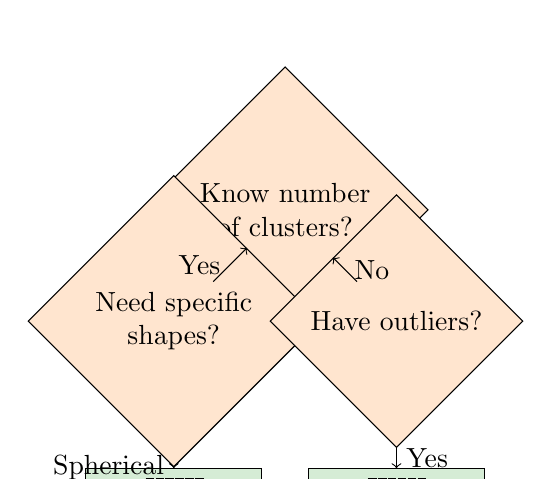
\begin{tikzpicture}[
    node distance=2cm,
    decision/.style={diamond, draw, text width=2.5cm, align=center, fill=mlorange!20},
    algo/.style={rectangle, draw, text width=2cm, align=center, fill=mlgreen!20},
]
\node[decision] (start) {Know number of clusters?};
\node[decision, below left of=start] (shape) {Need specific shapes?};
\node[decision, below right of=start] (outlier) {Have outliers?};
\node[algo, below of=shape] (algo1) {\_\_\_\_\_\_};
\node[algo, below of=outlier] (algo2) {\_\_\_\_\_\_};

\draw[->] (start) -- node[left] {Yes} (shape);
\draw[->] (start) -- node[right] {No} (outlier);
\draw[->] (shape) -- node[left] {Spherical} (algo1);
\draw[->] (outlier) -- node[right] {Yes} (algo2);
\end{tikzpicture}
\end{center}
\end{discoverybox}

\begin{casestudy}
\textbf{Amazon's Real Implementation:}
\begin{itemize}
\item Uses K-means on 100+ features for customer segmentation
\item Segments: Prime Power Shoppers, Deal Seekers, Brand Loyalists, Window Shoppers, One-time Buyers
\item Each segment receives different homepage layouts, email campaigns, and recommendations
\item Result: 35\% increase in conversion rate
\end{itemize}
\end{casestudy}

\newpage

% PAGE 8: Build Your Innovation Radar
\section*{Your Innovation Clustering Project}

\begin{exercisebox}{mlpurple}{Design Your Own Innovation Analysis}
Choose your field and complete this template:
\end{exercisebox}

\begin{discoverybox}{mlblue}{1. Your Innovation Domain}
\textbf{Field:} $\square$ Tech $\square$ Healthcare $\square$ Education $\square$ Finance $\square$ Other: \_\_\_\_\_

\textbf{20 Innovations in Your Field:}
\begin{multicols}{2}
\begin{enumerate}
\item \hrulefill
\item \hrulefill
\item \hrulefill
\item \hrulefill
\item \hrulefill
\item \hrulefill
\item \hrulefill
\item \hrulefill
\item \hrulefill
\item \hrulefill
\item \hrulefill
\item \hrulefill
\item \hrulefill
\item \hrulefill
\item \hrulefill
\item \hrulefill
\item \hrulefill
\item \hrulefill
\item \hrulefill
\item \hrulefill
\end{enumerate}
\end{multicols}
\end{discoverybox}

\begin{discoverybox}{mlorange}{2. Feature Selection}
\textbf{10 Key Features to Track:}
\begin{multicols}{2}
\begin{enumerate}
\item \hrulefill
\item \hrulefill
\item \hrulefill
\item \hrulefill
\item \hrulefill
\item \hrulefill
\item \hrulefill
\item \hrulefill
\item \hrulefill
\item \hrulefill
\end{enumerate}
\end{multicols}
\end{discoverybox}

\begin{discoverybox}{mlgreen}{3. Success Metrics}
\textbf{Target number of clusters:} \_\_\_\_\_

\textbf{Minimum silhouette score:} \_\_\_\_\_

\textbf{Business question to answer:} \hrulefill
\end{discoverybox}

\newpage

% PAGE 9: Reflection and Key Learnings
\section*{Your Discovery Reflections}

\begin{discoverybox}{mlpurple}{What Patterns Are You Missing?}
\textbf{Before today, I grouped innovations by:}

\hrulefill

\textbf{Now I realize I should also consider:}

\hrulefill

\hrulefill
\end{discoverybox}

\begin{challenge}
\textbf{The 270-Dimension Challenge}

If each innovation has 270 features, and you can only visualize 3 at a time, how many different 3D views would you need to see all possible combinations?

\textbf{Answer:} $\binom{270}{3} = \frac{270!}{3!(270-3)!} = 3,241,350$ views!

\textbf{Time to view all (at 1 second each):} 37.5 days non-stop!

\textbf{Time for ML to analyze all:} < 1 second
\end{challenge}

\begin{discoverybox}{mlblue}{Your Top 5 Discoveries}
\begin{enumerate}
\item \hrulefill
\vspace{0.3cm}
\item \hrulefill
\vspace{0.3cm}
\item \hrulefill
\vspace{0.3cm}
\item \hrulefill
\vspace{0.3cm}
\item \hrulefill
\end{enumerate}
\end{discoverybox}

\begin{casestudy}
\textbf{Success Story: Procter \& Gamble}
\begin{itemize}
\item Used clustering on 200+ innovation features
\item Discovered "Sustainable Millennials" segment
\item Launched Tide Eco-Box based on cluster insights
\item Result: \$100M new revenue stream in year 1
\end{itemize}
\end{casestudy}

\newpage

% PAGE 10: Action Plan and Resources
\section*{Your Innovation Clustering Action Plan}

\begin{discoverybox}{mlgreen}{Week 1 Action Items}
$\square$ Identify 50 innovations in your field\\
$\square$ List 20 features that matter\\
$\square$ Collect data for at least 10 innovations\\
$\square$ Try manual clustering with 3 features\\
$\square$ Calculate distances between top 5 innovations\\
$\square$ Identify which algorithm fits your needs
\end{discoverybox}

\begin{didyouknow}
\textbf{Industry Clustering Applications You Use Daily:}
\begin{itemize}
\item \textbf{Netflix:} 76,897 micro-genres from clustering viewing patterns
\item \textbf{Spotify:} 5,000 "taste clusters" for Discover Weekly
\item \textbf{Amazon:} 150 customer segments for personalization
\item \textbf{Google:} 2 billion web pages organized via clustering
\item \textbf{LinkedIn:} 147 skill clusters for job matching
\item \textbf{Instagram:} 32 interest clusters for Explore page
\end{itemize}
\end{didyouknow}

\begin{discoverybox}{mlcyan}{Resources to Explore}
\textbf{Interactive Demos:}
\begin{itemize}
\item www.tensorflow.org/playground - See clustering in action
\item projector.tensorflow.org - Visualize high-dimensional data
\item distill.pub/2016/misread-tsne/ - Understand dimensionality
\end{itemize}

\textbf{Real Datasets to Try:}
\begin{itemize}
\item Startup Database: www.crunchbase.com
\item Innovation Rankings: www.globalinnovationindex.org
\item Patent Database: patents.google.com
\end{itemize}
\end{discoverybox}

\begin{center}
\begin{tcolorbox}[colback=mlpurple!10, colframe=mlpurple!50, width=0.9\textwidth]
\centering
\Large \textbf{Final Challenge}\\[0.5cm]
\normalsize You've discovered that ML can find patterns in 270 dimensions that humans can't see.\\[0.3cm]
\textbf{Question:} What innovation opportunities might be hiding in YOUR data?\\[0.3cm]
Next week: We'll use these techniques on real innovation datasets!
\end{tcolorbox}
\end{center}

\vspace{1cm}

\begin{center}
\textbf{Course Instructors} | ML for Innovation | Week 1 Complete
\end{center}

\end{document}